\chapter{Facility Layer \label{chap:facilitylayer}}
\section{Komponenten}
\begin{figure}[htbp]
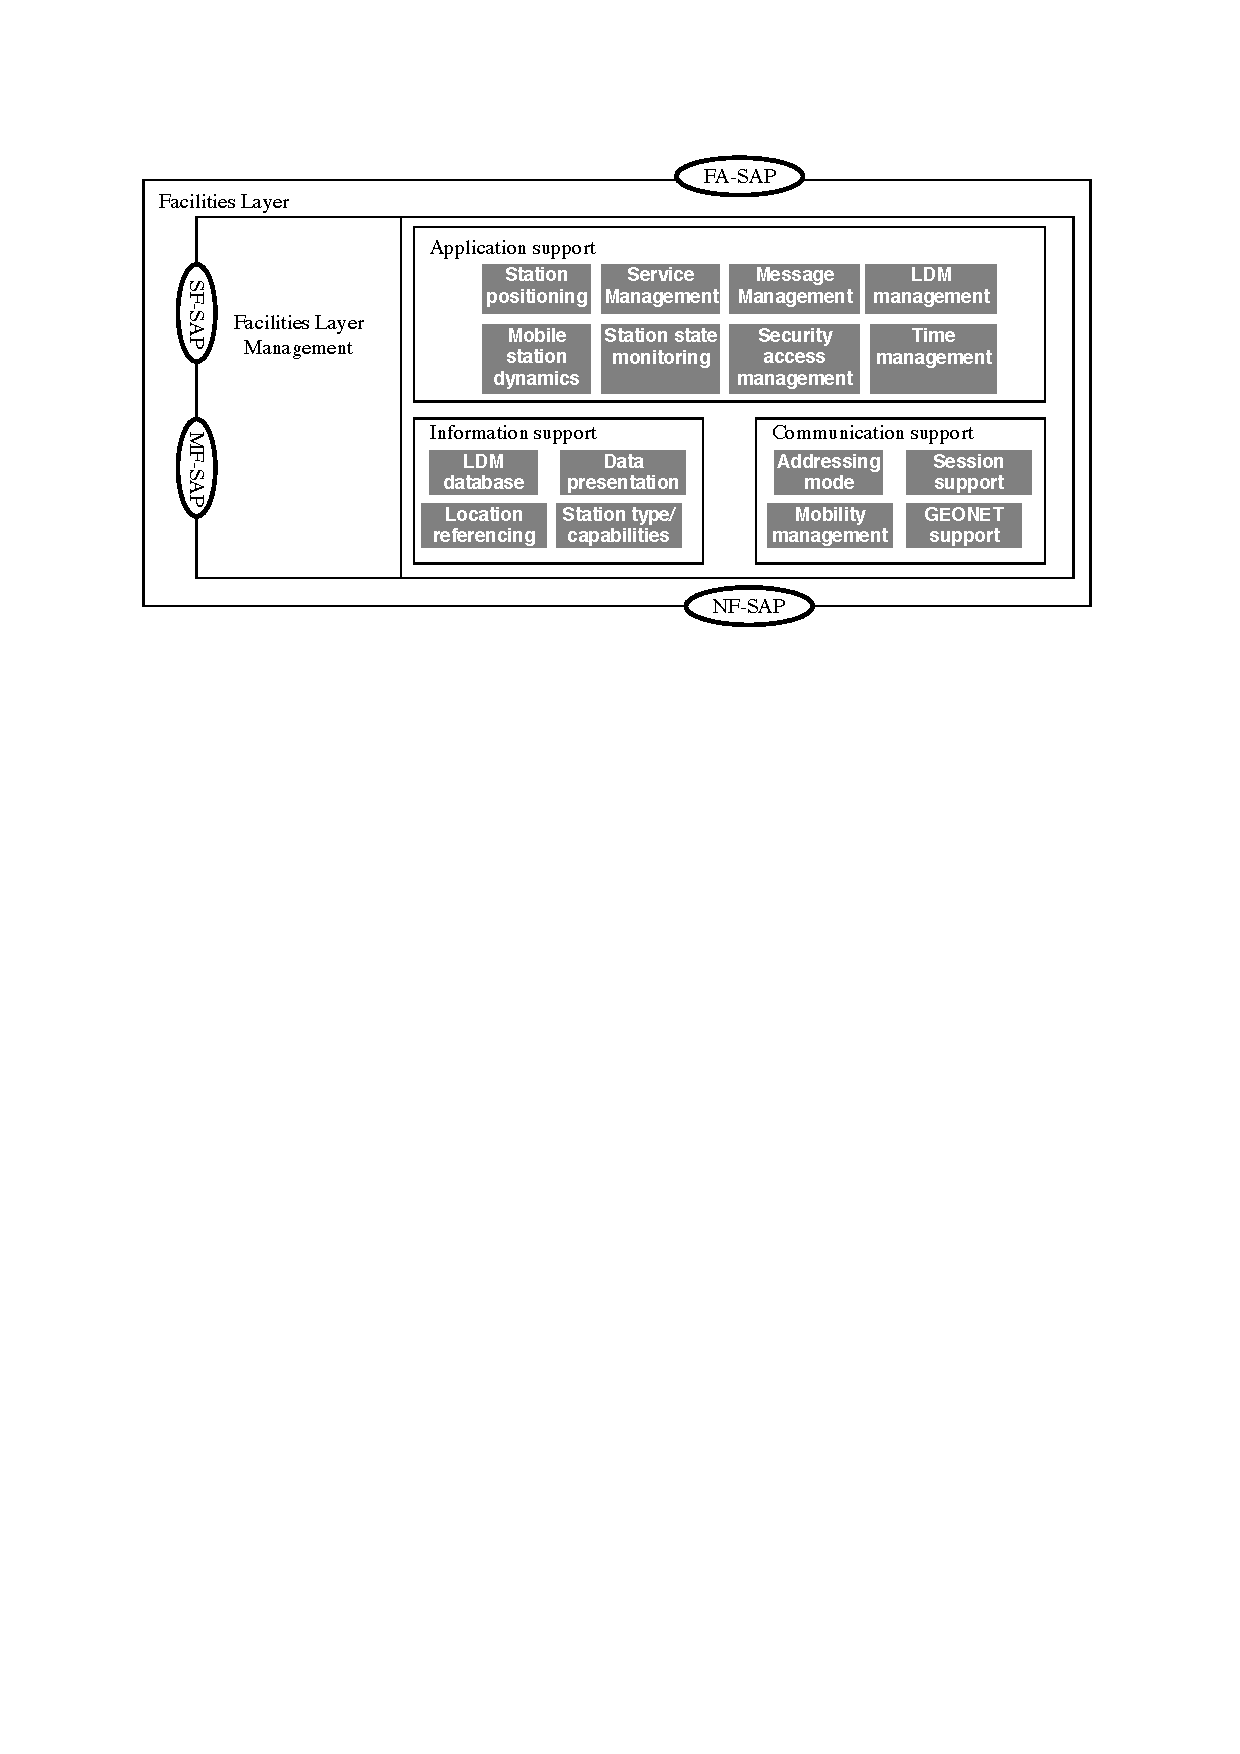
\includegraphics[width=0.99\textwidth]{content/images/04_facilitylayer/facility_layer_model.pdf}
\caption{Die Komponenten der \acl{C2C}}
\label{fig:komponentenfacility}
\end{figure}
Der Facility Layer liegt unterhalb des Applicationlayer und teilt sich in drei Hauptkomponenten auf. Er bietet verschiedene allgemeine Services an die von den Anwendungen des Application Layer verwendet werden können.

\subsection{Application Support}
Der Application Support stellt die Grundfunktionalität für die Anwendungen zur verfügung. Darunter fällt das station lifecycle management, das automatische erkennen von Services sowie das downloaden und initialisieren von neuen Services und noch weitere. Die einzelne Komponenten des Application Support, die auf der \autoref{fig:komponentenfacility} zu sehen sind, werden im folgenden genauer erläutert. 

\subsubsection{Station positioning}
Dieser teil des Application Support verarbeitet die Informationen die aus den verschiedenen Datensammler gewonnen werden wie aus GNSS oder aus Fahrzeugsensoren um die Position des Station zu gewinnen. 
Da diese Angaben sehr genau sein müssen werden die Daten in 3D Position gemessen (latitude, longitude, altitude). Dies können, durch beispielsweise GPS, in Echtzeit zur verfügung stehen. Da es jdeoch Sicherheitsbedingte Anwendungen gibt bei denen bereits über 0.5m Abweichung eine fatale Auswirkung haben kann, werden die Standortinformationen noch einmal über weitere Einheiten verbessert. Dazu gehören z.b. Odometer oder Gyroskop.
Damit diese Support facility ihren Aufgaben Nachkommen kann, ist im \cite{etsi102638} folgende Vorraussetzungen definiert.

\begin{itemize}
\item Benötigt Verbindung zwischen ITS station und einem GNSS system. Bei kurzfristigen Ausfall der Verbindung übernehmen interne mechanische Fahrzeugsensoren wie das Gyroskop oder das Odometer.
\item Benötigt dauerhafte Verbindung zu den Fahrzeugsensoren (direkte Verbindung oder über einen Bus).
\item Benötigt genug Rechenleistung um 3D Positions Angaben sicher zu Verwalten und zu Berechnen.
\end{itemize}

\subsubsection{Mobile station dynamic monitoring}
Das Mobile station dynamic monitoring ist nur für die \acs{VS} verfügbar. Diese Einheit des Facility Layer verwaltet eine große Anzahl an Fahrzeugspezifischen Daten die von den Applicationen und anderen Komponenten des Facility Layers verwendet werden. Sie ist dafür verantwortlich diese Daten immer auf dem neueste  Stand zu halten. 
Diese Einheit benötigt die folgenden Vorraussetzungen.

\begin{itemize}
\item Benötigt zugriff auf Fahrzeug Funktionen wie das Bremssystem, Reifendruck, Stabilitätskontrolle, Geschwindigkeitsregelung etc.
\item Muss verschiedne Parameter filtern können, die für die Applications benötigt werden (z.b Hauptzylinderdruck, Lenkradwinkel, Lenkradwinkeländerungsrate, Gierrate, Fahrzeuggeschwindigkeit oder Beschleunigungssteuerung).
\item Muss über die Möglichkeit besitzen die verschiedene Werte zu aktualisieren, die für die \acl{CAM} benötigt werden.
\end{itemize}

\subsubsection{Station state monitoring \label{facilitylayer_StationStateMonitoring}}
Die Station state monitoring facility überwacht dauerhaft den aktuellen Zustand eines Fahrzeuges. Diese können sich je nach Typ des Fahrzeuges unterscheiden. Bei einem Motorrad würde neben Lichtkontrolle, der Neigungswinkel interessant sein, wobei bei einem Rettungswagen der Status der Sirene mehr Sinn ergibt. Über diese Facility können solche Daten dauerhaft abgerufen werden. 
Dazu benötigt diese die folgenden Punkte.
\begin{itemize}
\item Benötigt Zugriff auf die verschiedene Funktionen die überwacht werden sollen (Motor / Antriebsstrang, Cockpit, Scheibenwischer, Lichtsteuerung, etc.).
\item Muss über die Möglichkeit verfügen diese Funktionen die von den Applications verwendet werden nach aktivität zu filtern.
\item Muss über die Möglichkeit besitzen die verschiedene Werte zu aktualisieren, die für die \acl{CAM} benötigt werden.
\end{itemize}

\subsubsection{Services management \label{facilitylayer_ServicesManagement} }
Da davon auszugehen ist das die verschiedenen Services im laufe der Zeit immer weiterentwickelt werden, muss es eine Einrichtung geben, über die die Services aktuell gehalten werden. 
Also is die Services management facility dafür da die Services auf dem neusten Stand zu halten, zu entfernen oder neue anzubieten. Die einzelnen Services werden von Services provisioning servers angeboten und können über eine spezielle Software direkt auf die ITS geladen werden. Damit dieser Vorgang durchgeführt werden kann, sind folgende Vorraussetzungen zu erfüllen.
\begin{itemize}
\item Die Services provisioning servers müssen die Fähigkeit besitzen für einzelne Services zu werben und die Lizenzbedingungen zu übermitteln. Der Zugang kann direkt über ein eigenes Globales Netzwerk geschehen oder indirekt über eine Roadstation bzw. einen Hotspot.
\item Die angebotenen Services werden über Nachrichten gesendet, diese müssen empfangen und analysiert werden können.
\item Um mit dem Benutzer zu interagieren müssen die ausgewählten Services an den Applicationlayer weitergegeben werden können um diese dem Benutzer zu präsentieren und dieser dann die Auswahl treffen kann.
\item Die Anwendunge müssen aktualisierbar sein um Bugs oder Fehler zu beheben.  
\end{itemize}

\subsubsection{LDM management \label{facilitylayer_LDMManagement}}
Die LDM management facility analysiert dauerhaft die Nachrichten die von dem Applicationlayer gesendet werden. Diese Änderungen werden in der LDM Database gespeichert und aktualisiert. Die LDM Database wird in \autoref{facilitylayer_ldmdatabase} genauer erläutert. Das heisst das alle Nachrichten die im gesamten C2X Netzwerk empfangen werden ausgewertet werden. Unter diesem befinden sich nicht nur Fahrbahninformationen über beispielsweise Kurven, Radwege oder Ampelsteuerungen sondern auch Informationen über die Objekte die über die Sensoren erkannt werden. Das führt zu einer sehr hohen Datenmenge die in der LDM Database verwaltet werden muss. Damit die LDM management dies tun kann sind folgende Voraussetzungen zu erfüllen.
\begin{itemize}
\item Die facility muss die einkommenden Nachrichten analysieren können und mit den relevanten Daten in Echtzeit die Datenbank aktualisieren.
\item Es muss eine leistungsfähige Datenbanksoftware zum Einsatz kommen die eine sehr große Menge an Daten verwalten kann und mit Zugriff von vielen Applications zurecht kommen muss.
\item Für Safety Applications muss gewährleistet sein das die relevanten Daten für die Application schnell selektiert werden können.
\item Muss die Daten für alle Anwendungen, die den Zugriff auf die LDM database benötigen, freigeben.
\end{itemize}

\subsubsection{Messages management \label{facilitylayer_MessagesManagement}}
Diese facility ist dafür da Nachrichten zu generieren, formatieren und zu strukturieren. Dies alles geschieht nach dem Europäischen Standart für diese Nachrichtentypen. Darunter zählen aktuell CAN und DENM, die in \autoref{sec:cam} und \autoref{sec:den} genauer erläutert werden. Darüber hinaus analysiert die facility die einkommenden Nachrichten und leitet deren wichtigen Inhalt an die anfordernden Applications weiter. Allerdings auch an andere lokale facilitys wie z.b. an die LDM management facility. Damit die Nachrichten richtig manipuliert werden können, sind in \cite{etsi102638} folgende Punkte aufgeführt.
\begin{itemize}
\item Nachrichten erstellen nach dem Europäischen Standart. 
\item Nachrichten erstellen die nach zukünftigen Europäischen Standart definiert sind.
\item Muss Nachrichten senden, stoppen oder weiterleiten, je nach Applicationanforderung.
\end{itemize}

\subsubsection{Security access management \label{facilitylayer_AccessManagement}}
Die Security access management facility als Kommunikationspartner für die Security Entity. Auf \autoref{fig:komponentenfacility} ist der SF-SAP erkennbar. Über diesen Access Point kommunizieren die beiden Layer miteinander und tauschen hier Informationen aus die für die Security wichtig sind. \todo{hier eventuell noch bischen mehr schreiben.}

\subsubsection{Time management \label{facilitylayer_TimeManagement}}
Um im gesamten System eine einheitliche Zeitreferenz zu besitzen, stellt die Time management facility diese zur verfügung. Diese Referenzzeit wird für Zeitstempel benutzt und kann von jeder Schicht abgerufen werden. Desweiteren  berechnet die Time management facility die maximale Latenzzeit einer Übertragung. Diese Information ist vor allem für zeitkritische Anwendungen von Interesse.
Damit die Facility richtig Arbeiten kann sind nachfolgende Anforderungen gestellt.
\begin{itemize}
\item Muss die Latenzzeit berechnen können, die benötigt wird bis eine Nachricht bei dem Networklayer ankommt. 
\item Die facility muss jeder Anwendung die sagen können, wie lange es dauert bis der Networklayer erreicht ist. 
\end{itemize}

\subsection{Information Support}
Der Information Support stellt die Präsentationsebene des \acs{ISO} \acs{OSI} Modells dar. Sie ist für die Datenverwaltung verantwortlich. Dazu gehören statische wie dynamische Daten, die meistens Gebiets- und Zeitabhängig sind und über eine Time to Live verfügen, also nicht für immer gültig sind. Um all diese Daten zu verarbeiten und immer auf dem aktuellen Stand zu halten ist im gesamten der Information Support verantwortlich. Die wichtigste Komponente hierbei ist die \acl{LDM}. Im folgenden wird auf alle einzelnen Komponenten des Information Support eingegangen. 

\subsubsection{LDM database \label{facilitylayer_ldmdatabase}}

\subsubsection{Data presentation}

\subsubsection{Location referecing}

\subsubsection{Station type/capabilities}

\subsection{Communication Support}
The communication support, which includes the session layer of the OSI Reference model. It will
cooperate with the transport and network layer to achieve the various communication modes required by
the applications. 

\section{CAM\label{sec:cam}}
\ac{ITS} bietet die Möglichkeit, dass \ac{ITS-S} untereinander Statusinformationen austauschen. Für den Austausch von Statusinformationen werden \ac{CAM} versandt. Diese beinhalten Informationen über die Anwesenheit allgemein, über die Position und den grundsätzlichen Status. Gemäß Standard \cite{ts102637-2} soll jede \ac{ITS-S} den Umgang mit diesen Nachrichten beherrschen. Das beinhaltet das Senden, das Empfangen und das Generieren dieser Nachrichten. So kennt jede \ac{ITS-S} ihre aktuellen Nachbarn inklusive ihrer Positionen, Bezwungen und den grundlegenden Sensorinformationen. Die \ac{CAM} werden über den Standard \ac{ITS-G5} übertragen. \ac{CAM} werden mit einer Kadenz zwischen 1 und 10 Hz übertragen, das bedeutet, dass mindestens jede Sekunde eine \ac{CAM} generiert und versendet wird, maximal werden aber 10 \ac{CAM} pro Sekunde generiert und versendet. Der Versand erfolgt über ein Single Hop Broadcast. \ac{CAM} spielen besonders für \ac{IVS} eine Rolle.

Die Verwaltung der \ac{CAM} findet im \ac{CAM} Management statt. Es hat Interfaces zu den anderen Facilities:
\begin{itemize}
	\item Station State Monitoring, \autoref{facilitylayer_StationStateMonitoring} (Bietet den aktuellen Staus der \ac{ITS-S} an)
	\item Mobile Station Dynamic Monitoring (Bietet Echtzeitkinematik der \ac{ITS-S} an)
	\item Time Management, \autoref{facilitylayer_TimeManagement} (Bietet eine global gültige Zeitreferenz für das markieren von Nachrichten an)
	\item Local Dynamic Map Management, \autoref{facilitylayer_LDMManagement}
\end{itemize}

Die anderen Facilities sind in der \autoref{fig:komponentenfacility} eingezeichnet. 

Das Nennen des vollständigen Inhalts einer \ac{CAM} würde den Rahmen dieser Ausarbeitung sprengen. Im Folgenden werden dennoch einige interessante Datenelemente aufgezählt. Sie entstammen dem Standard \cite{ts102637-2}. Dort können auch die Restlichen nachlesen werden.

\begin{itemize}
	\item \textbf{stationCharacteristics: } Dieses Datenelement besteht laut der \ac{ASN.1} Beschreibung aus mindestens drei weiteren Datenelemten:
	\begin{itemize}
		\item mobileItsStation: Kann die \ac{ITS-S} ihre Station ändern?
		\item privateItsStation: Die \ac{ITS-S} wird von keiner Behörde betrieben.
		\item physicalRelevantItsStation: Kann eine andere \ac{ITS-S} diese \ac{ITS-S} rammen?
	\end{itemize}
	\item \textbf{AmbientAirTemperature: } Die Außentemperatur, die die \ac{ITS-S} misst.
	\item \textbf{CrashStatus: } Dieses Datenelement enthält Informationen über einen Unfall, der eine Weiterfahrt verhindert. Beispiele dafür sind das Auslösen der Airbags oder ein Überschlag.
	\item \textbf{CurvatureChange: } Dieses Datenelement beschriebt die Änderung der Kurvenrichtung. Ein positiver Wert bedeutet, dass das \ac{IVS} nach rechts abbiegt.
	\item  \textbf{DangerousGoods: } Dieses Datenelement beschreibt, ob und welches Gefahrgut  das \ac{IVS} transportiert.
	\item \textbf{StationWidth: } Dieses Element beschreibt die zulässige Gesamtbreite der \ac{ITS-S}. Die Breite ist mit einer Feinheit von 0,01m aufgelöst.
\end{itemize}

\subsection{PDU Header \label{facilitylayer_PduHeader}}
\todo{Was zum PDU header schreiben}The ITS PDU header shall be as specified in ETSI TS 102 894-2 [5]. Detailed data presentation rules of the ITS PDU header in the context of DENM shall be as specified in clause B.1.

\subsection{Aufbau der CAM}
Eine \ac{CAM} besteht aus verschiedenen Containern, die wiederum Container enthalten. Ein Container ist...\todo{Aufbau CAM beschreiben}

\section{DEN\label{sec:den}}
\subsection{Beschreibung von DEN \label{facilityLayer_beschreibungDEN}}
\ac{DEN} ist definiert um die \ac{RHW} Anwendungsfälle zu unterstützen.	Die \ac{RHW} Anwendung ist auf \ac{IVS} und \ac{ITS} verteilt. Sie ist eine aktive Straßensicherheit Anwendung. Sie verteilt Informationen über die Straßenverkehrsverhältnisse. Um die \ac{DEN} Informationen zu verteilen gibt es \ac{DENM}. Diese enthalten die relevanten Informationen und informieren die andren \ac{ITS-S}. Sie werden beim Eintreffen eines \ac{RHW} relevanten Ereignisses an alle \ac{ITS-S} verteilt, die durch dieses Ereignis betroffen sind. Während das Ereignis anhält, werden die \ac{DENM} verteilt. Das Verteilen endet nach einer festgelegten Zeit oder durch eine weitere \ac{DENM}, die eine andere beendet. In einer \ac{ITS-S}, die eine \ac{DENM} empfängt, wird geprüft, ob die Information für den Benutzer relevant ist. Abhängig der Relevanz wird sie angezeigt oder nicht. Ein Beispiel für eine \ac{DENM}, die nach einer festen Zeit ungültig wird, ist eine Notbremsung eines \ac{IVS}. Durch die Bremsung entsteht eine temporäre Gefahr. 


\subsection{DEN Management}
Auf der \autoref{fig:darstellungDenServices} sind die Komponenten von \ac{DEN} dargestellt. Darauf zu erkennen ist, dass der \ac{DEN} Basic Service aus das \ac{DEN} Management und die \ac{LDM} besteht. Die restlichen Komponenten unterstützen den Service. 

\begin{figure}[htbp]
	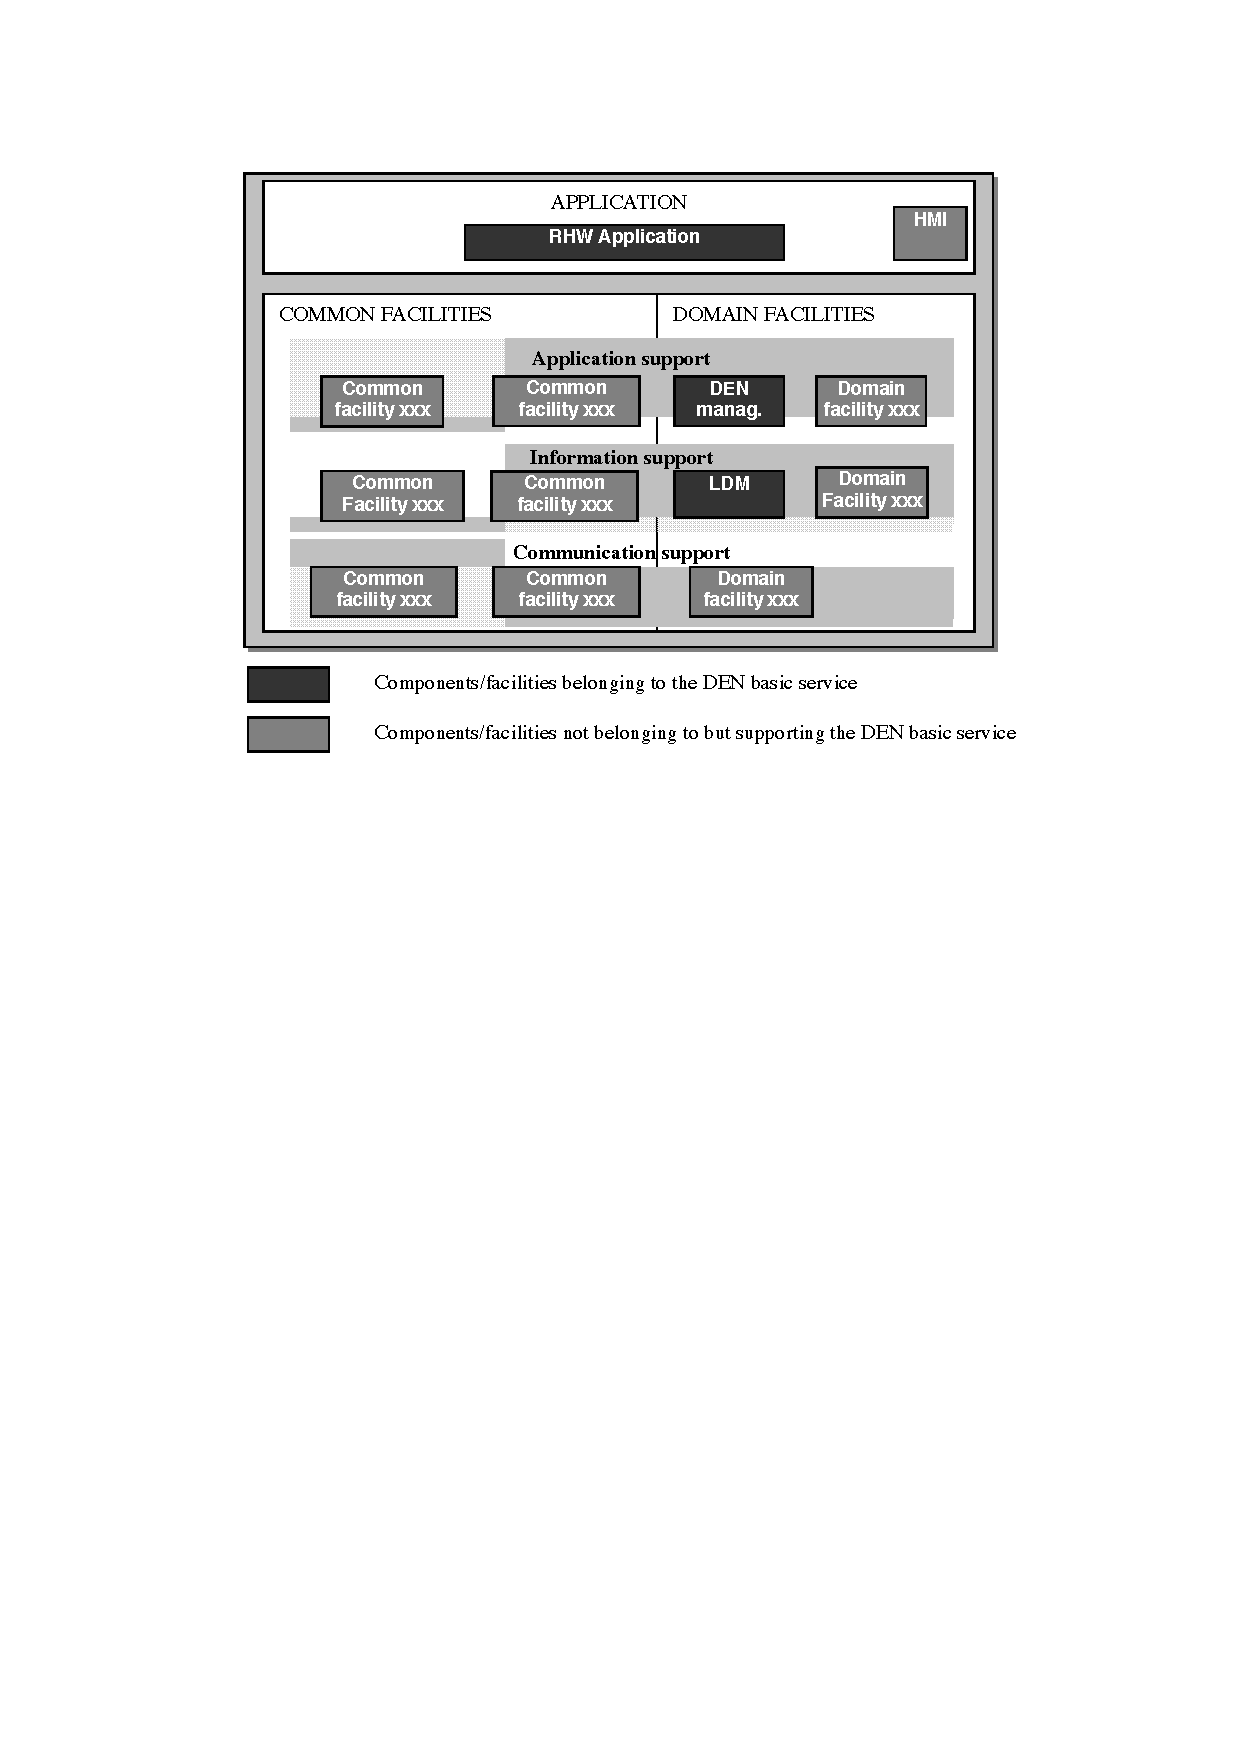
\includegraphics[width=0.95\textwidth]{content/images/04_facilitylayer/denServices.pdf}
	\caption{Service Komponenten von DEN \cite{ts102637-3}}
	\label{fig:darstellungDenServices}
\end{figure}


Das \ac{DEN} Management  ist für das Steuern der \ac{DENM} Übertragung verantwortlich. Dazu gehören das Gerieren, das Aktualisieren und das Beenden der Übertragung. Es regelt das \ac{DENM} Protokoll. Das schließt die Einhaltung des korrekten Nachrichtenformats und der korrekten Semantik ein. Zum erstellen von \ac{DENM} hat das \ac{DEN} Management Interfaces zu den \ac{RHW} Anwendungen und den anderen Facilities. Die \ac{DENM} werden in diesem Services auch aktuell gehalten. Veraltete \ac{DENM} werden gelöscht, bzw. für ungültig erklärt. Eine \ac{DENM}, die im \ac{DEN} Management erzeugt wird, muss mindestens den Typ des entdeckten Events und dessen Position enthalten. Zusätzlich muss sie die Eintrittszeit des Events und die voraussichtliche Dauer des Events enthalten. Kann keine voraussichtliche Dauer genannt werden, muss sie geschätzt werden. Das betroffene Gebiet muss auch genannt werden. Bei dem Gebiet, bzw. relevante area, handelt es sich um einen oder mehrere Straßenabschnitte, in denen sich die \ac{ITS-S} befinden die von dem Event betroffen werden. Ein Gebiet kann aber auch eine Richtung sein.

\subsection{DEN Basic Service}
Der \ac{DEN} Basic Service ist für die Verarbeitung von \ac{DENM} verantwortlich. Die Verarbeitung beinhaltet auf der sendenden Seite das Auslösen von \ac{DENM} und auf die der empfangenden Seite das Empfangen der \ac{DENM}, sowie deren Bereitstellen für die Benutzung in den \ac{ITS-S} Anwendungen. Das Auslösen kann in mehrere Tätigkeiten unterteilt werden und wird im Folgenden genauer erklärt. Der \ac{DENM} Basic Service kann auch die Funktionalität des Weiterleitens von \ac{DENM} anbieten. Der \ac{DEN} Basic Service besteht wiederum aus fünf weiteren Komponenten. Er hat fünf Interfaces. Die Komponenten und Interfaces sind in der \autoref{fig:darstellungDenBasicServiceKomponenten} abgebildet.

\subsubsection{Interfaces}
Mithilfe der Interfaces stellt der \ac{DEN} Basic Service seine Informationen zur Verfügung. Interfaces haben allgemein den Vorteil, dass die Funktionalitäten oder Layer nicht aufeinander abgestimmt werden müssen, sondern nur klar definierte Übergabepunkte implementieren müssen. Dadurch kann sich beispielsweise die Funktionalität des \ac{DENM} Versenden völlig ändern, ohne dass die Applications angepasst werden müssen. 

Der \ac{DEN} Basic Service hat fünf Interfaces. Davon bieten drei Interfaces Schnittstellen zu anderen Layern, zwei sind reine Daten Interfaces. Die Interfaces werden im Folgenden genannt und kurz erläutert. Die genaue Beschreibung und die Auflistung der zu übertragenden Daten  kann dem Standard \cite{en302637-3} entnommen werden.

\paragraph{IF.N\&T}
Das Interface IF.N\&T ist  eine Schnittstelle zum Network und Transport Layer. Als sendende \ac{ITS-S} übergibt der \ac{DEN} Basic Service über dieses Interface die \ac{DEMN} um sie zu versenden. Als Empfangender empfängt er die \ac{DENM} über dieses Interface. Wenn die \ac{DENM} versendet werden muss mindesten die \ac{DENM} selber sowie die Destiantion Area und das Repetition Interval übergeben werden. Die beiden Werte bestimmen, wohin die \ac{DENM} versendet werden soll und wie oft das Senden wiederholt werden soll. Wird eine \ac{DENM} empfangen, muss mindestens die empfangene  \ac{DENM} über das Interface übergeben werden.

\paragraph{IF.SEC}
Der Standard \cite{en302637-3} beschreibt zu diesem Interface lediglich, dass es Informationen zu dem Security Layer überträgt.  
\paragraph{IF.Mng}
Der Standard \cite{en302637-3} beschreibt zu diesem Interface lediglich, dass es Informationen zu dem Management Layer überträgt. 
\paragraph{IF.DEN.1}
Das Interface IF.DEN.1 wird vom Application Layer genutzt. Damit werden Anforderungen für \ac{DENM} übertragen. Möglich sind die Anforderungen AppDENM\_trigger, AppDENM\_update, AppDENM\_termination. Sie entsprechen dem Anfordern, dem Aktualisieren oder dem Beenden von \ac{DENM} und werden vom Application Layer an den \ac{DEN} Basic Service übertragen. Die übertragenen Daten sind im Standard \cite{en302637-3} definiert. Die Anfragen vom Application Layer werden vom \ac{DEN} Basic Service mit der actionId der bearbeiteten \ac{DENM} oder einer Fehlerbenachrichtigung quittiert.
\paragraph{IF.DEN.2}
Das Interface IF.DEN.2 wird genutzt um die empfangen Daten vom \ac{DEN} Basic Service in den Application Layer zu transportieren. Dabei werden ganze \ac{DENM} transportiert.


\subsubsection{Komponenten}
Die Komponenten des \ac{DENM} Basic Service erfüllen die Aufgaben des Basic Service.

\paragraph{Endode DENM \label{facilitylayer_EncodeDENM}}
Diese Komponente konstruiert eine \ac{DENM}. Dazu werden die zu übertragenden Daten kodiert. In dieser Komponente werden lediglich die vorhandenen Daten zu einer \ac{DENM} zusammengefasst. Die Kodierung erfolgt mithilfe von \ac{ASN.1} und ist im Standard \cite{en302637-3} beschrieben. 

\paragraph{Decode DENM}
Diese Komponente dekodiert die empfangenen \ac{DENM} und stellt somit die enthaltenen Daten bereit.

\paragraph{DENM transmission management}
Das Transfusion Management erfüllt die Aufgaben, die für das Versenden von \ac{DENM} nötig sind. Das Versenden beginnt bei der Erstellung einer \ac{DENM}. Die Erstellung wird von einer Application angefordert. Nachdem die \ac{DENM} erstellt wurde, wird sie von der Komponente \ref{facilitylayer_EncodeDENM} kodiert. Neben der Erstellung einer neuen \ac{DENM} können auch vorhandene \ac{DENM} aktualisiert werden. Dies geschieht auch in diesem Layer und läuft analog zu dem Erstellen neuer \ac{DENM}. Das Beenden von \ac{DENM} Übertragungen und die wiederholte Übertragung wird auch in dieser Komponente gemacht.

\paragraph{DENM reception management}
Das Empfangsmanagement stellt die Funktionalitäten des \ac{DENM} Empfangs bereit. Beim Empfangen werden die \ac{DENM} überprüft und verworfen, wenn sie ungültig sind. Wenn sie gültig sind werden sie in die Message Table eingetragen. Die Message Table speichert die empfangenen \ac{DENM}. Dabei werden \ac{DENM} mit der gleichen actionId nur einmal gespeichert. Es wird immer nur die aktuelle \ac{DENM} mit einer actionId gespeichert. Die message table muss mindestens aus den Folgenden Spalten bestehen:

\todo{Prüfen, ob die genannten Werte noch erklärt werden. Wenn nicht $\Rightarrow$ hier erklären}
\begin{itemize}
	\item actionID: Die actionID der \ac{DENM}, auf die sich die Zeile bezieht.
	\item referenceTime: Diese Spalte erhält die referenceTime der \ac{DENM}, die als letztes empfangen wurde. 
	\item termination: Diese Spalte enthält die termination Werte der gespeicherten \ac{DENM}
	\item detectionTime: Diese Spalte enthält die detectionTime Werte der gespeicherten \ac{DENM}
\end{itemize}
 
Das \ac{DENM} reception management stellt stellt die die Daten der empfangen \ac{DENM} den anderen Komponenten des Facility Layers und den Anwendungen zur Verfügung.

\paragraph{DENM Keep Alive Forwarding}
Das Keep Alive Forwaring implementiert das im \ac{DENM} Protokoll beschriebene Verfahren zum Weiterleiten dass die \ac{ITS-S} \ac{DENM} weiterleitet. Der Standard \cite{en302637-3} bezeichnet diese Komponente als optional. Ein genaues Protokoll zum Weiterleiten der \ac{DENM} ist noch nicht definiert.




\begin{figure}[htbp]
	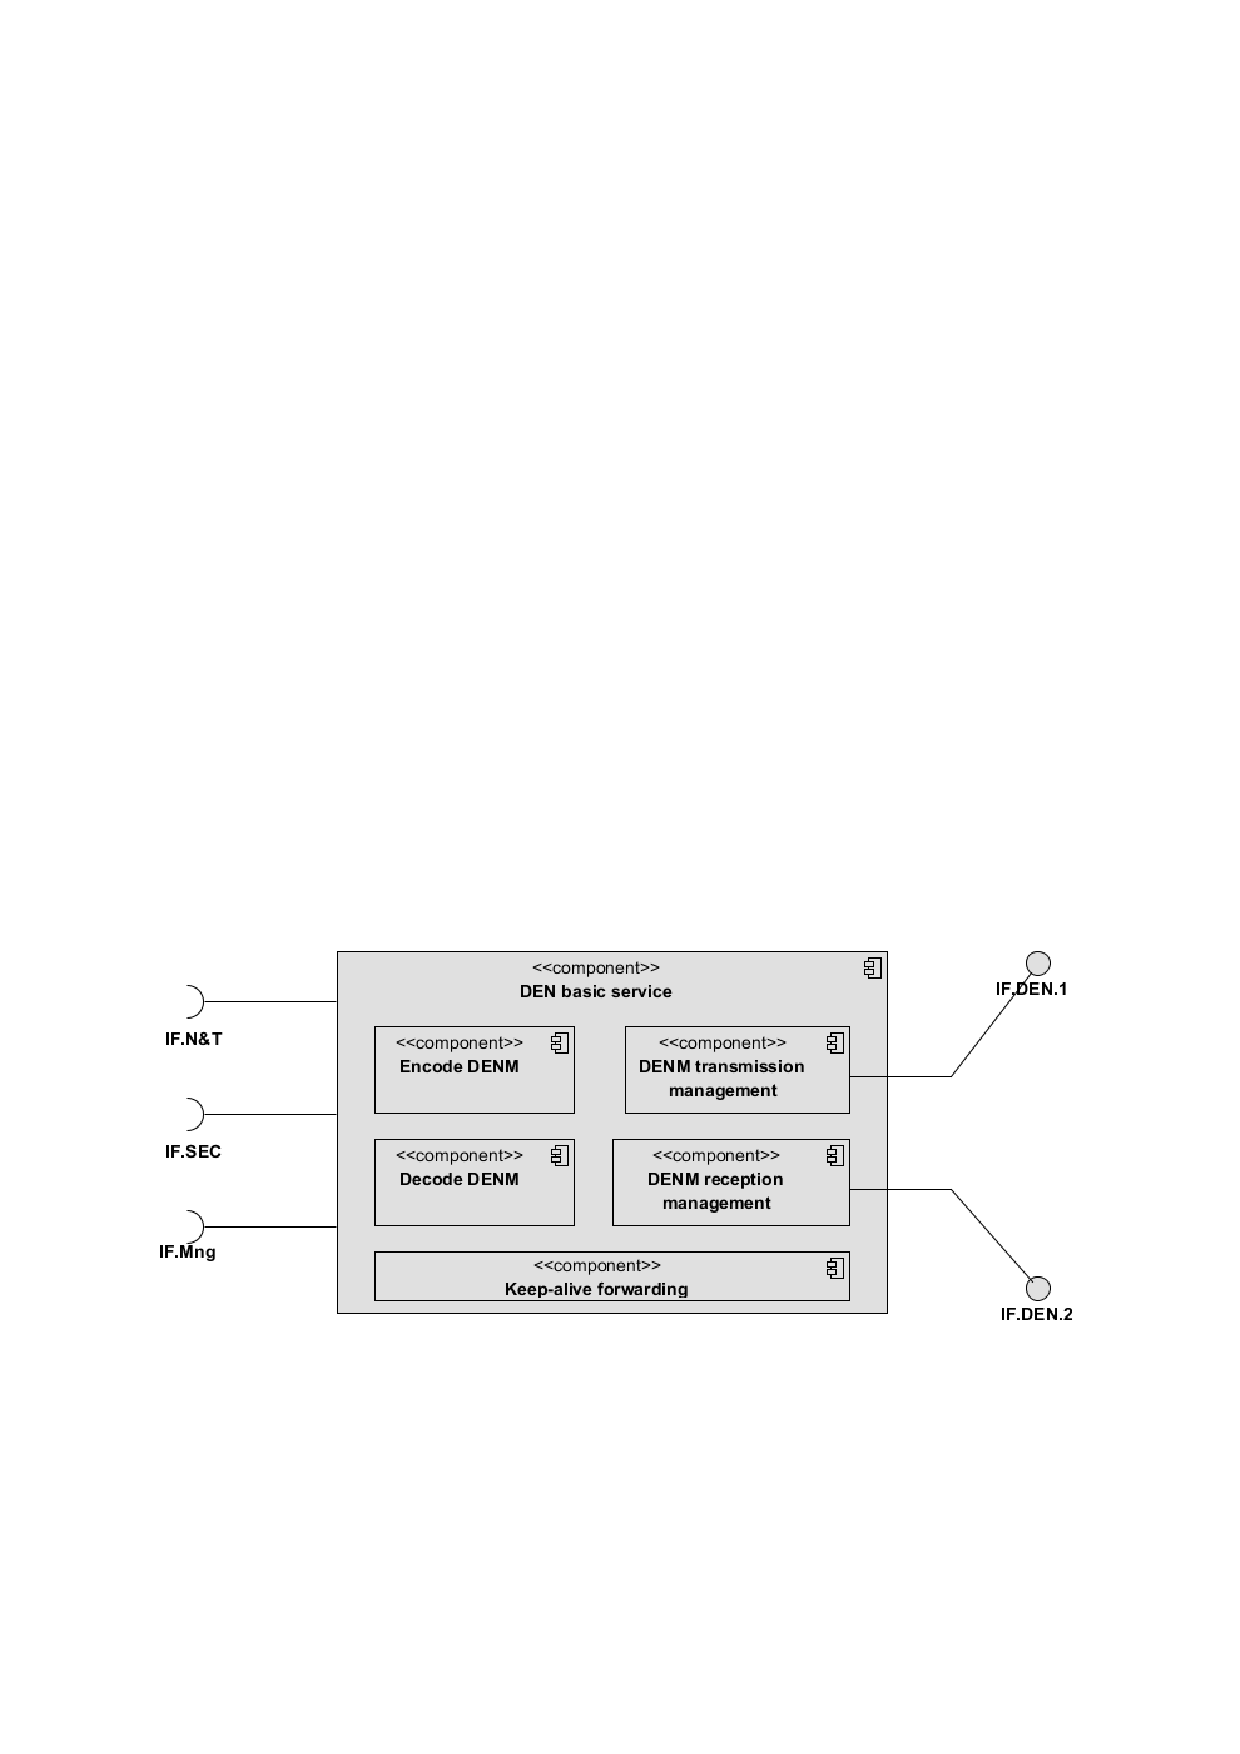
\includegraphics[width=0.75\textwidth]{content/images/04_facilitylayer/denBasicServiceKomponenten.pdf}
	\caption{Komponentendiagramm mit den Komponenten des DEN Basic Service \cite{en302637-3}}
	\label{fig:darstellungDenBasicServiceKomponenten}
\end{figure}

\subsection{Verbreitung der DENM}
Eine \ac{DENM} soll an so viele \ac{ITS-S} des gleichen Gebiets wie möglich verteilt werden. Das schließt auch \ac{ITS-S} ein, die während der Eventdauer das Gebiet erreichen. Auch wenn eine \ac{ITS-S} keine direkte Verbindung zu der auslösenden \ac{ITS-S} hat, soll sie die \ac{DENM} empfangen. Deswegen werden einige Parameter von der \ac{RHW} Applikation selber definiert. Die Liste dieser Parameter beginnt mit dem Zeitintervall zwischen den \ac{DENM}, die von der gleichen \ac{ITS-S} ausgesendet werden. Neben der Frequenz wird auch die maximale Latenz definiert, die für das Senden der \ac{DENM} benötigt wird und die Priorität der \ac{DENM}. Die Latenz beschreibt die Zeit, die \ac{DENM} vom Facility Layer der aussendenden \ac{ITS-S} zum Networking and Transport Layer der empfangenden \ac{ITS-S} zu senden. Die Priorität wird nicht in der \ac{DENM} selber festgelegt, da sie von unteren Layern übertragen wird. Das Zielgebiet für die \ac{DENM} wird auch von der \ac{RHW} Application festgelegt.


\begin{figure}[htbp]
	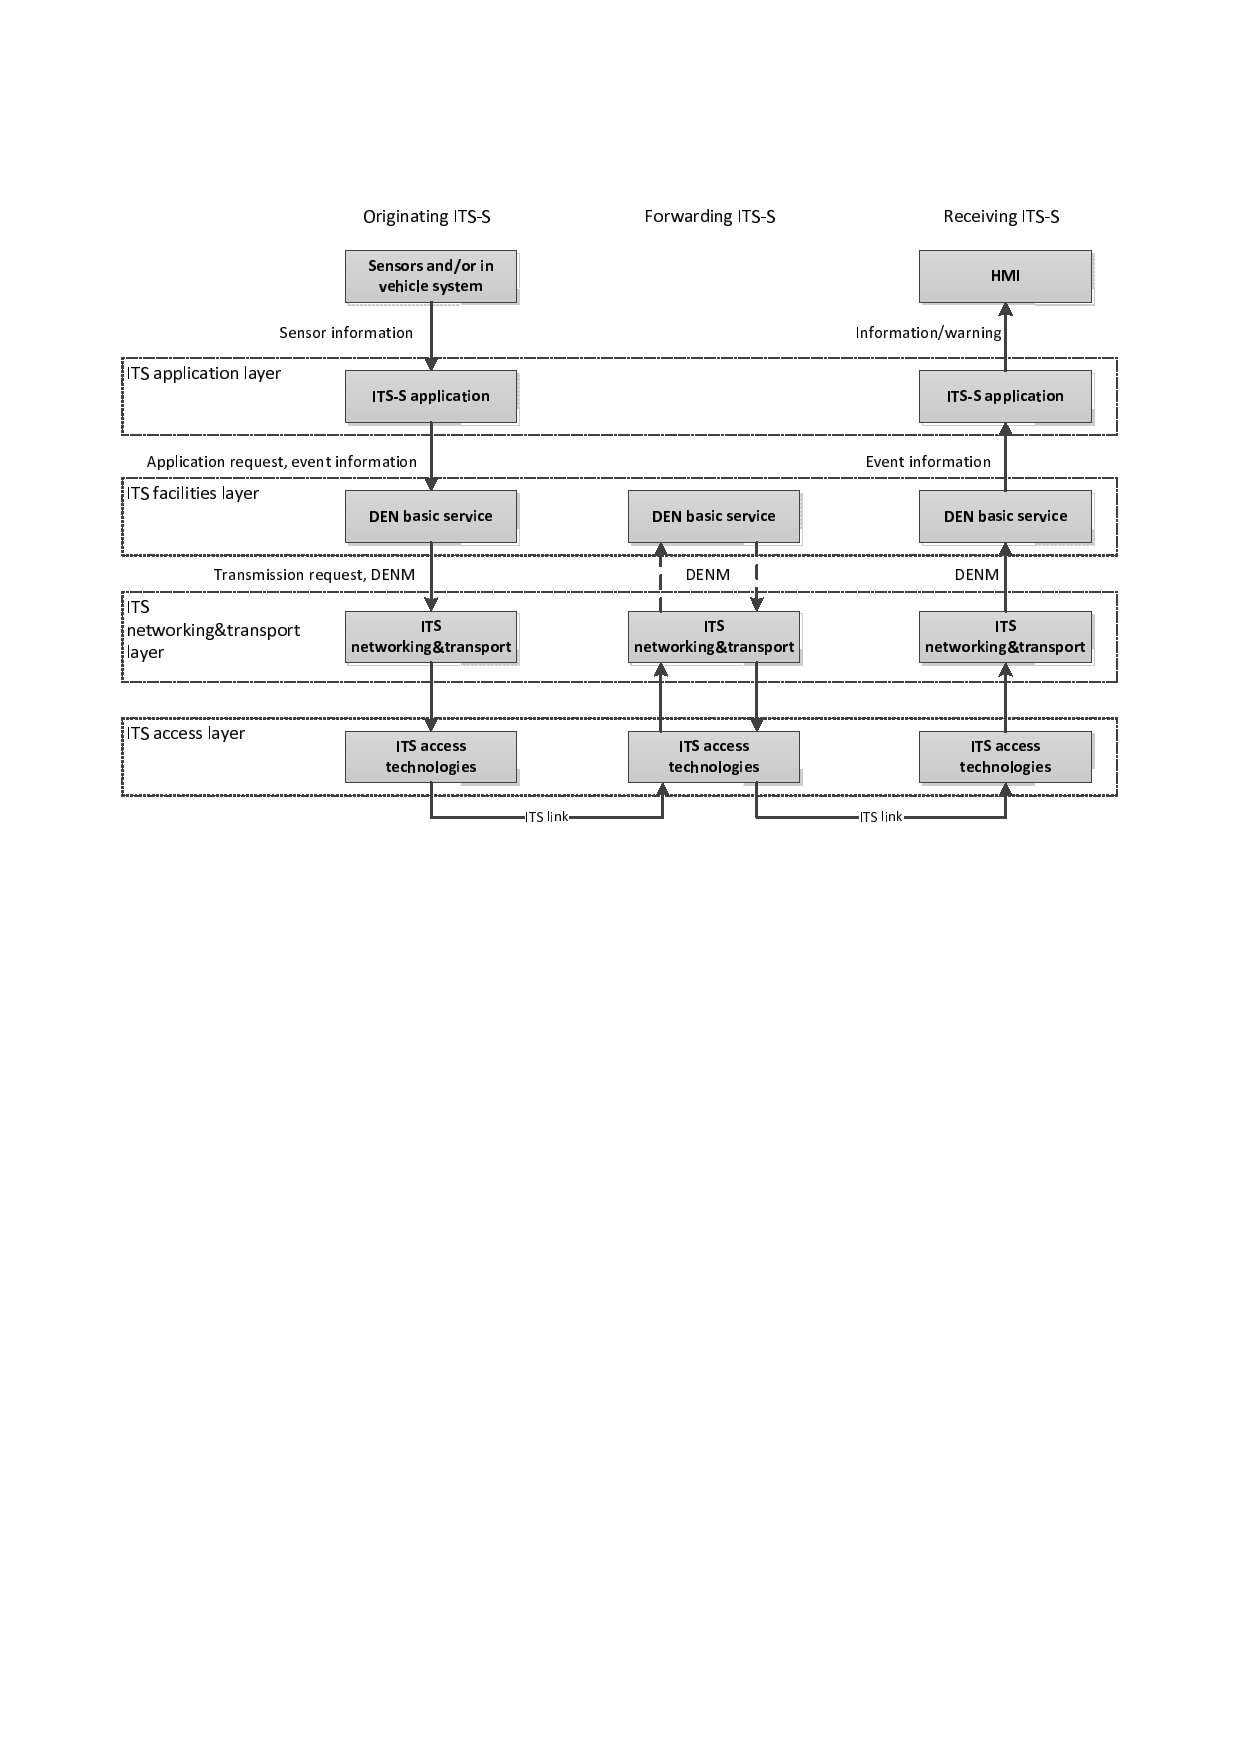
\includegraphics[width=0.99\textwidth]{content/images/04_facilitylayer/denVersendenLayerUeberblick.pdf}
	\caption{Datenfluss einer DENM über die Layer \cite{en302637-3}}
	\label{fig:darstellungDenVerteilenLayer}
\end{figure}

Die \autoref{fig:darstellungDenVerteilenLayer} zeigt, wie sich eine \ac{DENM} über die verschiednen Layer ausbreitet. In diesem Prozess sind drei \ac{ITS-S} beteiligt. Es gibt eine sendende \ac{ITS-S}, eine Empfangende und eine, die nur weiterleitet. Zu sehen ist, dass die Verarbeitung der \ac{DENM} im Application Layer beginnt und endet. Am Weiterleiten sind nur die unteren Layer, bis einschließlich der Facilities Layer beteiligt. Die Entscheidung, ob und wie weitergeleitet wird wird im \ac{DEN} Basic Service getroffen. 

\subsection{Die Aktualisierung von DENM}
Wenn sich ein Event, zu dem es bereits \ac{DENM} gibt, ändert, müssen die \ac{DENM} aktualisiert werden. Dazu gibt es das \ac{DENM} update.Das \ac{DENM} Update wird vom Application Layer angefordert und in \ac{DEN} Basic Service erstellt. Dieser Prozess wird von der \ac{ITS-S} angestoßen, die die \ac{DENM} ursprünglich versendet hat. Bei einem Update wird die referenceTime der \ac{DENM} aktualisiert, die actionID bleibt unverändert. 

\todo{DENM Update schreiben} 
 
\subsection{Die Beendung des Events}
\todo{Prüfen, ob die Wörter Cancellation und Negation genutzt werden. Wenn nicht $\Rightarrow$ eintragen.}
Bereits im \autoref{facilityLayer_beschreibungDEN} wurde beschrieben, dass ein Event entweder durch den Ablauf einer Zeit oder durch eine \ac{DENM}, die das Event beendet, beendet werden. Eine beendende \ac{DENM} kann entweder eine Annullierende oder eine Negierende sein. 

Die annullierende \ac{DENM} wird von der \ac{ITS-S} versendet, die das Ereignis ursprünglich bekannt gemacht hat. Sie wird versendet, wenn die \ac{ITS-S} feststellt, dass das Event beendet wurde.  Die annullierende \ac{DENM} ist eine \ac{DENM} mit einer speziellen Datenversion.

Die Negierende \ac{DENM} wird von \ac{ITS-S} gesendet, die das Event ursprünglich nicht angekündigt haben. Sie haben bereits \ac{DENM} zu dem Event empfangen und festgestellt, dass das Event nicht weiter existiert. Eine negierende \ac{DENM} enthält ein Negationsflag. 

Wenn eine beendende \ac{DENM} aus einer vertrauenswürdigen Quelle empfangen wurde, löscht das \ac{DEN} Management der empfangenden \ac{ITS-S} alle anderen \ac{DENM} zu dem gleichen Event. Die beendende \ac{DENM} muss, genau wie die Ankündigenden, eine Zeit lang weiter verteilt werden. Diese Zeit wird von der \ac{RHW} Application bestimmt.


\subsection{Aufbau der DEMN}
Eine \ac{DENM} besteht aus mehren Containern. Die Container sind in einer festen Reihenfolge angeordnet.  Vor den Containern befindet sich ein \ac{ITS} PDU Header, vgl. \autoref{facilitylayer_PduHeader}. Soweit der Aufbau der Datentypen beschrieben ist, werden sie beschrieben. Auffällig ist, dass der Standard \cite{en302637-3} wegen dem Aufbau der Datentypen auf den Standard \cite{ts102894-2} referenziert. Dieser beschreibt die Datenelement aber nicht immer.

\begin{figure}[htbp]
	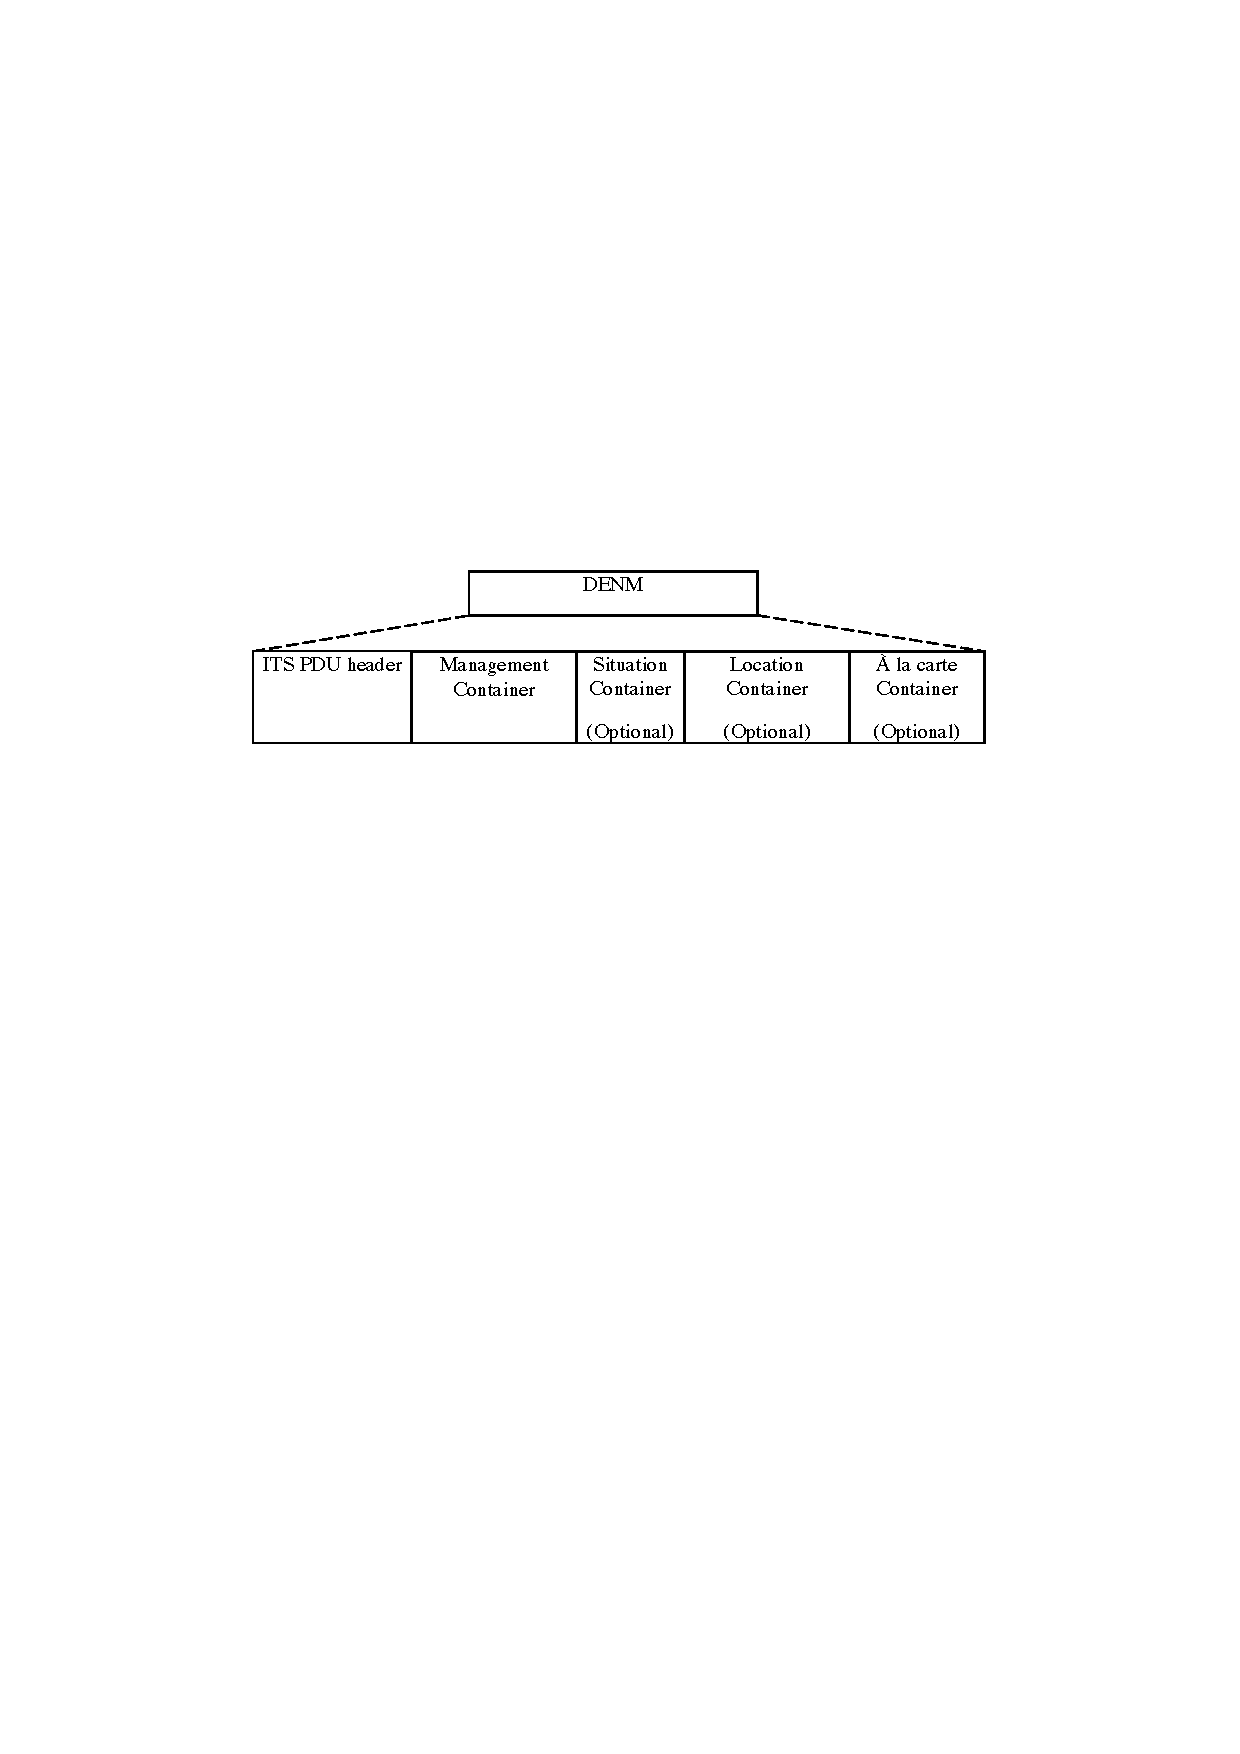
\includegraphics[width=0.95\textwidth]{content/images/04_facilitylayer/denmAufbau.pdf}
	\caption{Aufbau einer DENM \cite{en302637-3}}
	\label{fig:darstellungdenmAufbau}
\end{figure}

\subsubsection{Management Container}
Der Management Container enthält Management Daten des entdeckten Events und Informationen zum \ac{DENM} Protokoll. Er enthält die folgenden Daten:
\paragraph{actionID}
Die actionID identifiziert ein Event. Sie soll das Event einzigartig beschreiben und wird für jedes Event neu generiert und diesem zugewiesen. Sie besteht aus der \ac{ITS-S} \ac{ID} der erstellenden \ac{ITS-S} und einer Sequenzummer, die noch nicht benutzt wurde. Falls mehrere \ac{ITS-S} eine \ac{DENM} zu dem gleichen Event erstellen, müssen sich die actionID der \ac{DENM} unterscheiden. 

Die actionID einer \ac{DENM} ändert sich nicht mehr. Auch nicht, wenn die \ac{DENM} weitergeleitet oder aktualisiert wird. Anhand der actionID können die \ac{ITS-S} \ac{DENM} voneinander unterscheiden, die von unterschiedlichen \ac{ITS-S} zu einem gleichen Event erstellt wurden.

\paragraph{detectionTime \label{facilitylayer_referenceTime}}
Die detectionTime ist die Zeit, zu der das Event von der sendenden \ac{ITS-S} entdeckt wurde. Diese Zeit wird geändert, wenn eine \ac{DENM} aktualisiert wird, oder wenn das Event beendet wird. Gemäß Standard \cite{ts102894-2} ist die Zeit als die Millisekunden seit 00:00:00.000 01. Januar 2004 \ac{UTC} definiert.

\paragraph{referenceTime}
Die referenceTime ist die Zeit, zu der die \ac{DENM} erstellt wurde. Sie ändert sich bei Updates und Cancel \ac{DENM}. Der Darstellungstyp der Referenzen wurde im \autoref{facilitylayer_referenceTime} beschrieben.

\paragraph{termination}
Dieses Datenelement bestimmt, ob die generierte \ac{DENM} ein Cancellation oder eine Negation \ac{DENM} ist. Es wird nur mitgesendet, wenn die \ac{DENM} eine Cancellation oder eine Negation \ac{DENM} ist. 

\paragraph{eventPosition}
Dieses Element beschreibt die geographische Position des entdeckten Events. Die Position wird von der entdeckenden \ac{ITS-S} bestimmt. Wenn die meldende \ac{ITS-S} ein \ac{IVS} ist, soll als Position die Position gewählt werden, zu der sich das \ac{IVS} zum Zeitpunkt befand, als es das Event entdeckt hat. Im Standard \cite{ts102894-2} beinhaltet die ReferencePosition den Breitengrad, den Längengrad, die Höhe und die positionConfidenceEllipse. Letztere beschreibt die horizontale Genauigkeit.


\paragraph{relevanceDistance}
Dieses Element beschreibt den Umkreis, wie weit das gemeldete Event Einfluss auf \ac{ITS-S} hat. Dieses Element ist optional. 

\paragraph{relevanceTrafficDirection}
Dieses Element beschreibt die Fahrtrichtung, in der das Event für \ac{ITS-S} interessant ist. Dieses Element ist optional. 

\paragraph{validityDuration}
Dieses Datenelemet   beschreibt, wie lange die \ac{DENM} gültig ist, bzw. das Event dauert. Anhand dieses Elements wird die \ac{DENM} aus dem \ac{DEN} Basic Service gelöscht. Wenn die Dauer des Events nicht bestimmt werden kann, wird ein Defaultwert gesetzt. Die \ac{ITS-S}, die das Event gemeldet hat, kann die Zeit verlängern.  

\paragraph{transmissionInterval}
Dieses Datenelement beschreibt, in welchem Intervall das \ac{DENM} Senden wiederholt werden soll. Es wird von der meldenden \ac{ITS-S} gesetzt. Wenn es nicht gesetzt wurde, leiten die anderen \ac{ITS-S} die \ac{DENM} nicht weiter. 

\paragraph{stationType}
Dieses Datenelement beschreibt den Typ der sendenden \ac{ITS-S}. Die vordefinierten Typen sind für \ac{IVS} ausgelegt. Der Wert wird als Ganzzahl übertragen. Im Standard \cite{ts102894-2} sind  16 Werte vorbelegt, die Zahl kann maximal den Wert 255 annehmen.


\subsubsection{Situation Container}
Der Situation Container enthält Daten zu dem entdeckten Event. Er muss mindestens die Datenelemente informationQuality und eventType beinhalten. Darüber hinaus kann er aber noch weitere Elemente enthalten. Die Informationen, die hier übertragen werden, werden vom Application Layer bereit gestellt.

\paragraph{informationQuality}
Dieses Datenelement beschreibt die Wahrscheinlichkeit, ob das entdeckte Event wirklich passiert ist. Es wird von der entdeckenden Application gesetzt. Dieses Element ist eine Ganzzahl und kann acht Werte annehmen, wobei 0 unbekannt bedeutet, der niedrigste Wert ist 1 und der höchste Wert ist 7.

\paragraph{eventType \label{facilitylayer_eventType}}
Der eventType beschreibt das Event, das entdeckt wurde. Der eventType besteht wiederum aus mehreren Werten. Der erste Wert ist nennt sich causeCodeType und enthält den Grund des Events. Beispiele hierfür sind accident,  wrongWayDriving oder vehicleBreakdown. Er ist als Ganzzahl codiert und besitzt einen Zahlenraum von 256. Der zweite Wert des eventTypes ist der SubCauseCodeType. Er ist auch eine Anzahl mit dem Wertebereich 0..255. Der subCauseCode beschreibt den causeCode genauer, eine genauere Beschreibung ist zum gegenwärtigen Zeitpunkt nicht in den \ac{ETSI} Dokumenten zu finden.

\paragraph{linkedCause}
Dieses Datenelement beschreibt ein verknüpftes Event. Es enthält die gleichen Werte wie der eventType, vgl.  \ref{facilitylayer_eventType}. Ein Beispiel für ein verknüpftes Event ist ein vehicleBreakdown, das der linkedCause für ein dangerousEndOfQueue ist.  



\paragraph{eventHistory}
Dieses Datenelement beschreibt eine Liste von Event Positionen. Es kann verwendet werden, um ein weiträumiges Event, wie z.B. 9 Hazardous location - Surface condition, genauer zu beschrieben. Dazu können bus zu 40 Punkte des gleichen Events beschrieben werden, an denen das \ac{IVS} vorbeigekommen ist.


\begin{figure}[htbp]
	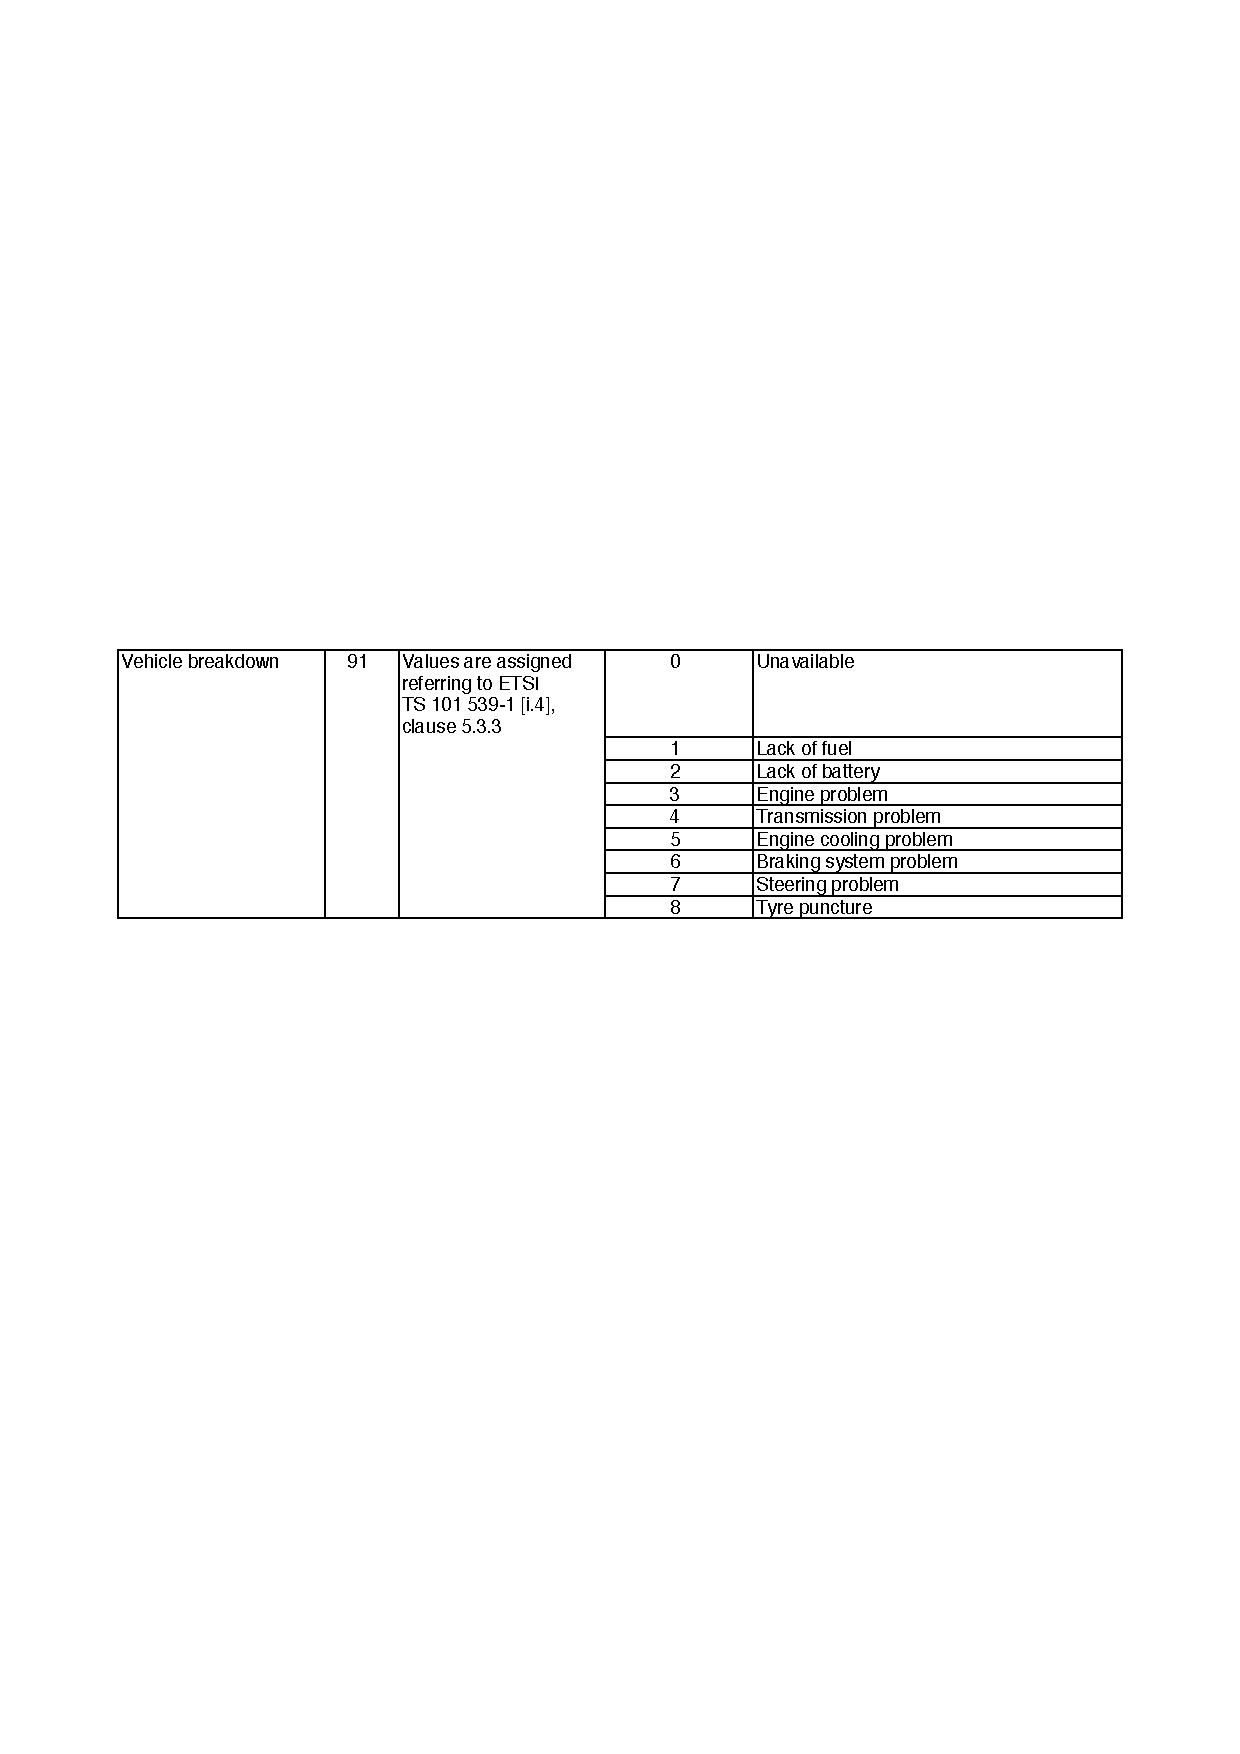
\includegraphics[width=0.95\textwidth]{content/images/04_facilitylayer/denmCauseCodeBeispiel.pdf}
	\caption{Beispieldaten für Cause Codes \cite{en302637-3}}
	\label{fig:causeCodeBeispiele}
\end{figure}


Die \autoref{fig:causeCodeBeispiele} zeigt einen Ausschnitt aus dem Standard   \cite{en302637-3}. Darin ist eine Zuordnung von causeCode und subCauseCode beschrieben. Das vorliegende Beispiel zeigt den causeCode 91, also ein defektes Fahrzeug. Zu diesem causeCode sind neun subCauseCodes aufgelistet, die den Grund des Defekts beschreiben, wie z.B. der subCauseCode 3, Motorprobleme.  

\subsubsection{Location Container}
Der Location Container enthält die Informationen zur Position des entdeckten Events. Neben der reinen Position des Events kann er auch andere Datenfelder enthalten.

\paragraph{eventSpeed}
Dieses Datenelement beschreibt die Geschwindigkeit des entdeckten Events. Zusätzlich wird die genau der Geschwindigkeitsmeldung mitgesendet. 

Die Genauigkeit wird in in 127 Wegen codiert, wobei der Wert 1 \glqq withinOneCentimeterPerSec\grqq~bedeutet und der Wert 126 \glqq outOfRange\grqq~bedeutet. 

Die Geschwindigkeit selber wird von \glqq standstill(0)\grqq~über\glqq oneCentimeterPerSec(1)\grqq~bis \glqq unavailable (16383)\glqq~kodiert. Die Einheit ist $0,01 \frac{m}{s}$.

\paragraph{eventPositionHeading}
Dieses Datenelement beschreibt die Fahrtrichtung des Events und die Genauigkeit dieser Information. 

Die Fahrtrichtung wird als Gradzahl beschrieben, die vom in WGS84 definierten Norden abhängt. Die Auflösung der Richtung ist 0,1 Grad. Norden entspricht 0 Grad, Süden entspricht dem dem Wert 1800.

Die Genauigkeit der Richtung wird mit einem Wert zwischen 0 und 127 beschrieben. 0 entspricht \glqq withinZeroPointOneDegree (0)\geqq~und der Wert entspricht \glqq unavailable (127)\grqq.

\paragraph{traces}
Das Datenelement traces beinhaltet mehrere Wegpunkte. Sie bilden zusammen eine Wegbeschreibung zu dem Event. Eine \ac{DENM} kann mehre Trasse enthalten. Dadurch können verschiedene Wege zu dem Event beschrieben werden. Ein \ac{IVS} kann seine eigene Route mit den empfangen Trasse vergleichen und feststellen, ob es auf dem Weg zum Event ist. Aktuell darf eine \ac{DENM} bis zu sieben traces enthalten.


\paragraph{roadType}
Das Datenelement roadtype beschreibt den typ der Straße. Möglich sind vier Werte, es wird unterschieden, ob die Fahrspuren getrennt sind und ob es eine städtische Straße ist oder nicht. 


\section{SPaT\label{sec:spat}}
\ac{SPaT} ist eine Nachricht, die den Zustand einer Straßenkreuzung beschreibt. Die Beschreibung enthält Staus Informationen der \ac{VBA} und Informationen über die Kreuzung selber. \ac{SPaT} ist noch nicht von der \ac{ETSI}, bzw. \ac{ISO} standardisiert. Aus diesem Grund stammen die folgenden Informationen hauptsächlich aus den U.S. amerikanischen Quellen \cite{usSpat} und \cite{usCaliforniaSpat}. 

Für \ac{SPaT} gibt es zwei grundsätzliche Betriebsarten. Die erste Betriebsart ist eine feste \ac{VBA} Schaltung. Diese wird den \ac{IVS} über \ac{SPaT} Nachrichten mitgeteilt. Anhand dieser Informationen kann das \ac{IVS} selber die Ampelzeiten berechnen und benötigt keine  weiteren \ac{SPaT} Nachrichten. Die zweite Betriebsart ist, dass die Ampelzeiten aufgrund externer Ereignisse beeinflusst werden können. Externe Ereignisse sind beispielsweise Fußgänger, verkehrsabhängige Schaltungen oder periodisierte \ac{IVS}, wie z.B. Rettungswagen. Bei der zweiten Betriebsart muss beachtet werden, dass zu schnelle Änderungen vermieden werden müssen. Die \ac{IVS} benötigen eine bestimmte Zeit zur Reaktion, so benötigt beispielsweise ein Auto die Reaktionszeit des Fahrers und einen Bremsweg. Wird die Fahrspur dieses Autos gesperrt und andere Fahrspuren dafür freigegeben, wenn das Auto sich schon fast vor der Haltelinie befindet, so ist eine Bremsung vor der Kreuzung nicht mehr möglich. Daraus resultiert ein Sicherheitsrisiko, da die andere Fahrspur nicht für die anderen Fahrzeuge garantiert frei ist. \todo{Rausfinden, ob die \ac{IRS} die Position des \ac{IVS} verwertet und daraus die Zeiten generiert. S.29 US Department.. -> Ich glaube die verwendet die Daten}

Auf dieser Grundlage können weitere Dienste angeboten werden. So können Abbiegeassistent Systeme oder Vorzugsschaltungen realisiert werden. 

 Abbiegeassistent Systeme unterstützen \ac{IVS} beim Abbiegen in Kreuzungen. Anhand der Positions- und Geschwindigkeitsdaten der \ac{IVS} kann die \ac{IRS} berechnen, ob ein Abbiegen nach rechts oder nach links sicher ist. Neben der Positionsdaten können auch Erfassungssysteme genutzt werden, die in die Infrastruktur integriert sind. Beispiele hierfür können \ac{Radar} oder \ac{Lidar} Systeme genutzt werden. Der Nachteil von rein \ac{ITS} basierten Systemen ist, dass nicht \ac{ITS} kompatible Fahrzeuge nicht erkannt werden. Das bedeutet, dass die \ac{IRS} eine freie Kreuzung erkennt und meldet, obwohl nicht \ac{ITS} basierende Fahrzeuge über die Kreuzung fahren. 
 
Die Bevorzugung von Fahrzeugen bietet sich für die Empfehlung \cite{usSpat} für Notfallfahrzeuge, für Fahrzeuge des Nahverkehrs und für den Frachtverkehr an. Durch die Bevorzugung können diese \ac{IVS} eine grüne Welle erreichen. Das bedeutet, dass entweder Grünphasen verlängert werden oder Rotphasen unterbrochen werden. Sofern nicht bereits durch andere Nachrichten, wie \ac{CAM} geschehen, fordert das \ac{IVS} bei der \ac{IRS} eine Bevorrangung an, wenn anhand der \ac{SPaT} erkennt, dass die Kreuzung nicht frei ist. Die \ac{IVS} beantwortet diese Anfrage im positiven Fall mit einer weiteren \ac{SPaT} Nachricht, die eine freie Kreuzung signalisiert.   

Inhalt einer \ac{SPaT}:
\begin{longtable}{|c|c|}
 \hline
\textbf{Datenelemente} & \textbf{Typ/Größe}\\
 \hline
 \hline
Object ID & Unsigned 8 Bit Integer\\
 \hline
 Object Size& Unsigned 8 Bit Integer\\
 \hline
 Apptoach ID & Unsigned 8 Bit Integer\\
 \hline
 Signal Phase Indication &  32 Bit Bitmask \\
 \hline
 Countdown Timer Confidence & 32 Bit Bitmask \\
 \hline
 Time to Signal Phase Change (Countdown Time) & Unsigned 16 Bit Integer \\
 \hline
 Yellow Duration & Unsigned 8 Bit Integer\\
 \hline
 \caption{Inhalt einer SPaT Nachricht \cite{usSpat}}
 \label{tab:facilitylayer_inhaltSpatNachricht}
 \end{longtable}
 
\todo{Werte der Tabelle beschreiben oder den Mist löschen}
\begin{figure}[htbp]
	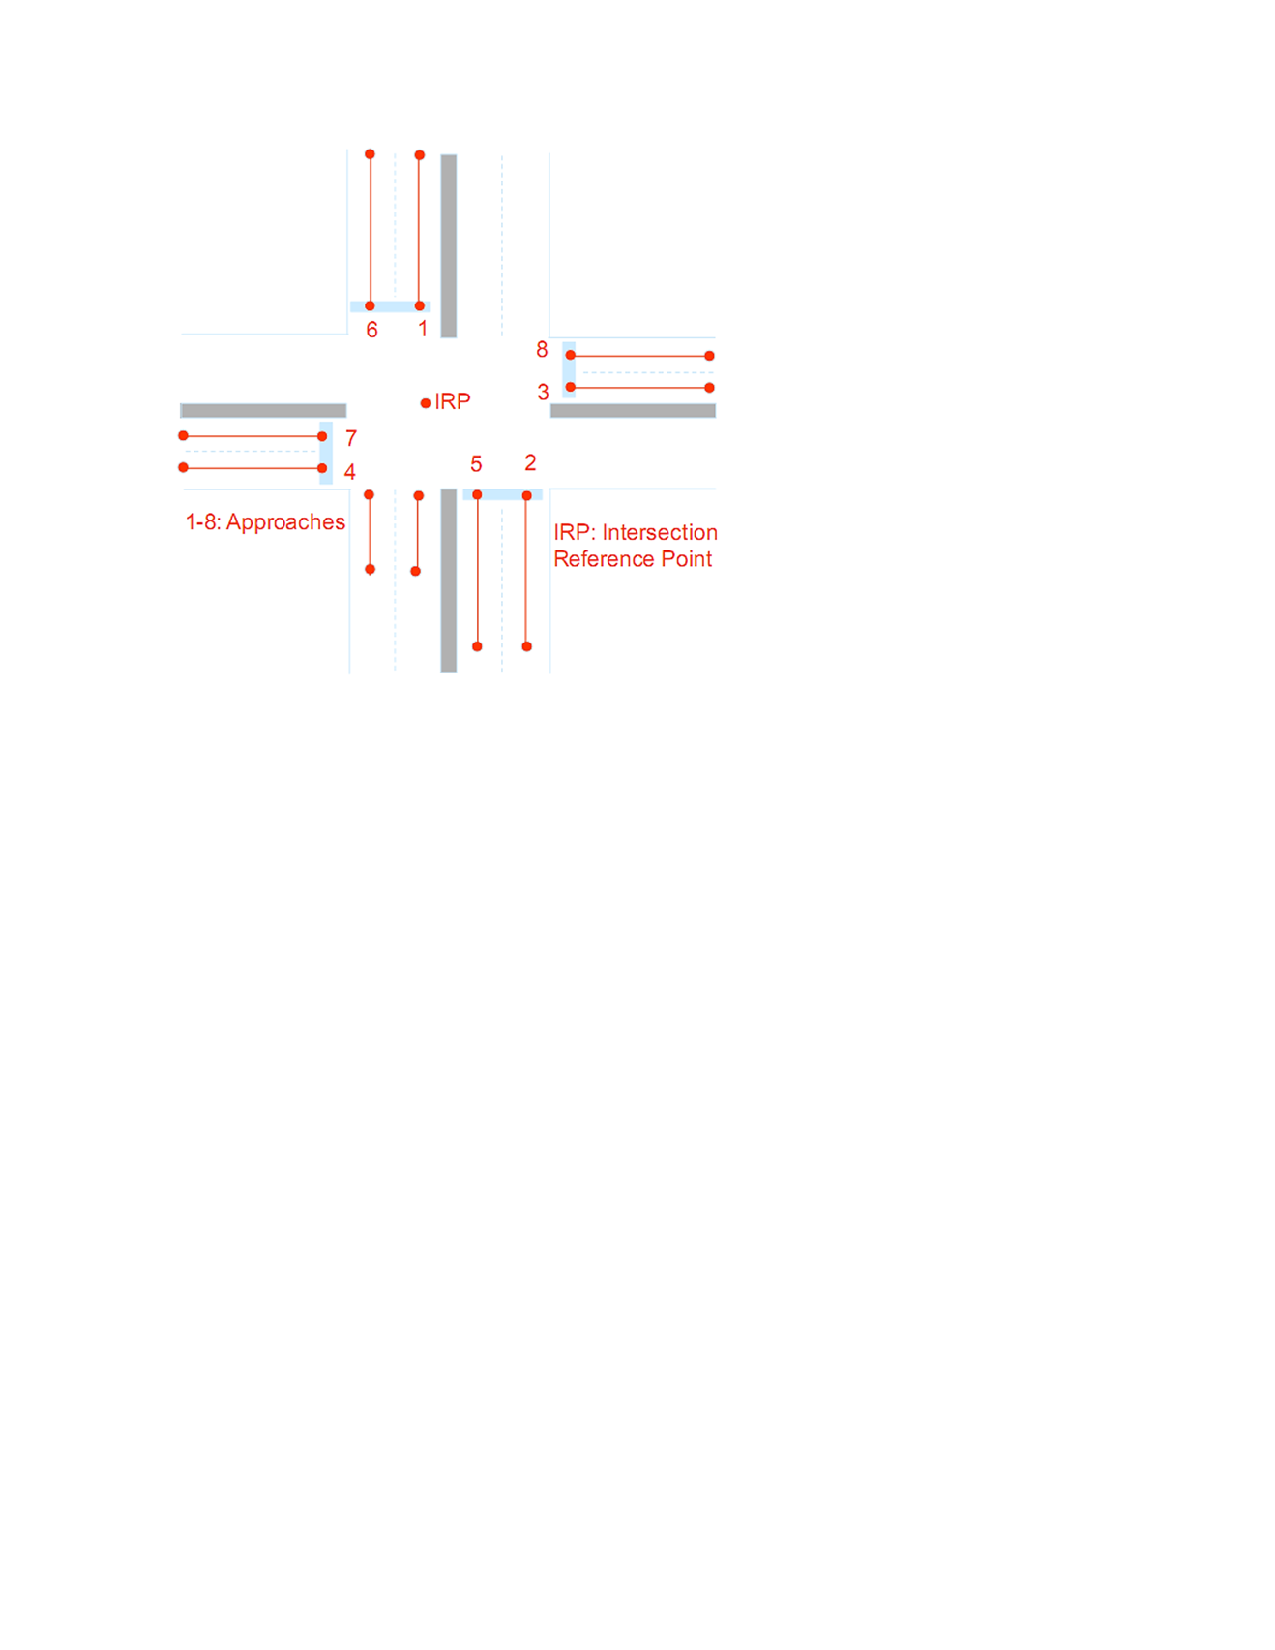
\includegraphics[width=0.60\textwidth]{content/images/04_facilitylayer/spatKreuzung-Anfahrtsstreifen.pdf}
	\caption{Kreuzung mit Darstellung der Approach ID \cite{usSpat}}
	\label{fig:darstellungKreuzung}
\end{figure}




\section{TOPO\label{sec:topo}}
